% ============================================================
% main.tex — Coronary Heart Disease Prediction Report
% Individual Coursework — Machine Learning
%
% Requirements:
%   - Max 1000 words, 5 pages
%   - Font size >= 12pt, margins >= 1 inch, 1.5 line spacing
%   - Compiled from the report/ directory:
%       pdflatex main.tex
%       bibtex main
%       pdflatex main.tex (x2)
% ============================================================

\documentclass[12pt,a4paper]{article}

% ── Page layout ───────────────────────────────────────────────────────────────
\usepackage[top=1in, bottom=1in, left=1in, right=1in]{geometry}

% ── Line spacing ──────────────────────────────────────────────────────────────
\usepackage{setspace}
\onehalfspacing

% ── PDF inclusion (submission form) ───────────────────────────────────────────
\usepackage{pdfpages}

% ── Typography & encoding ─────────────────────────────────────────────────────
\usepackage[T1]{fontenc}
\usepackage[utf8]{inputenc}
\usepackage{microtype}

% ── Tables & figures ──────────────────────────────────────────────────────────
\usepackage{booktabs}
\usepackage{graphicx}
\usepackage{float}
\usepackage{caption}
\usepackage{array}          % extended column formatting
\usepackage{wrapfig}        % text wraps around figures/tables

% ── Hyperlinks ────────────────────────────────────────────────────────────────
\usepackage[colorlinks=true, linkcolor=black, citecolor=blue, urlcolor=blue]{hyperref}

% ── References ────────────────────────────────────────────────────────────────
\usepackage[numbers,sort&compress]{natbib}
\usepackage{doi}            % clickable DOI hyperlinks

% ── ToC depth ─────────────────────────────────────────────────────────────────
\setcounter{tocdepth}{1}    % sections only — saves space

% ── Appendix ──────────────────────────────────────────────────────────────────
\usepackage[title]{appendix}

% =============================================================================
\begin{document}

% ── Page 1: Coursework Submission Form ───────────────────────────────────────
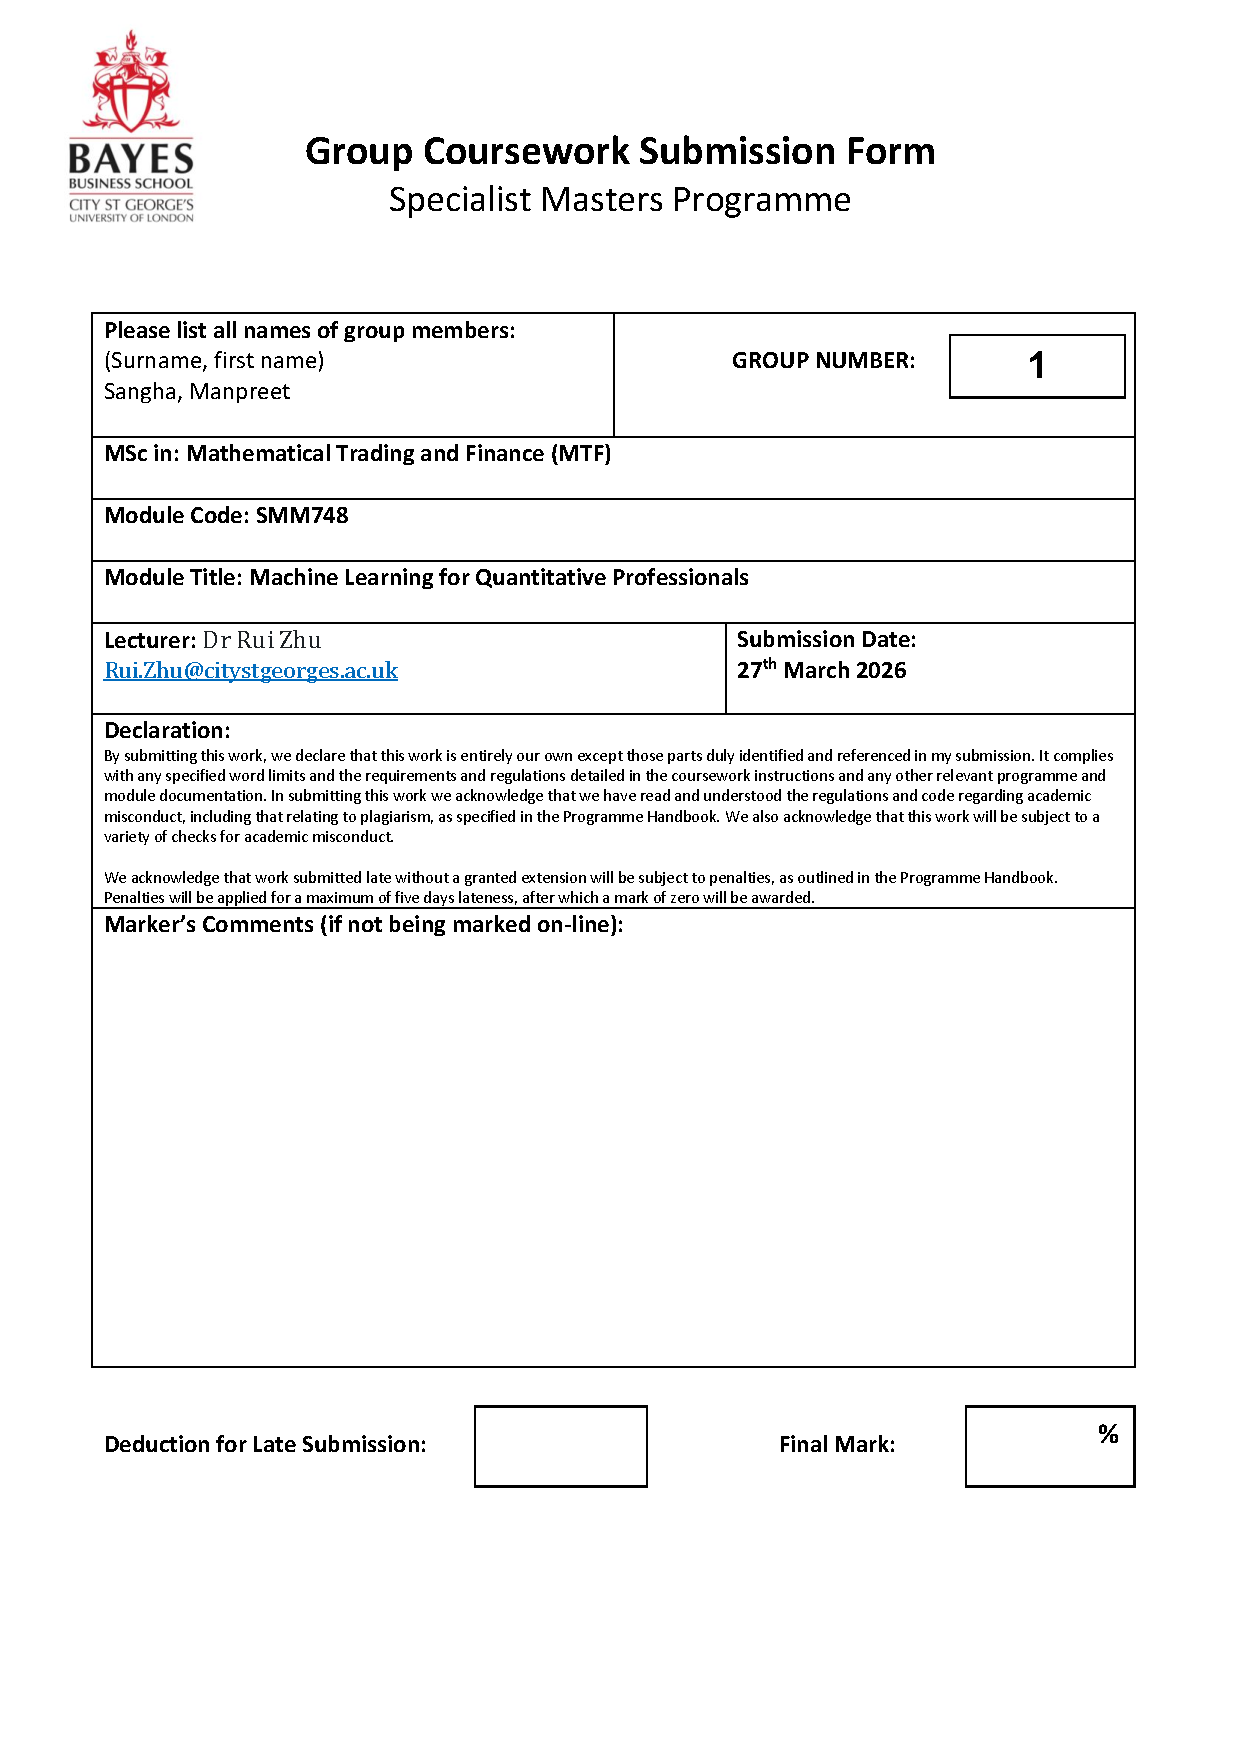
\includepdf[pages=1]{Group Coursework Submission Form.pdf}

% ── Table of Contents ─────────────────────────────────────────────────────────
\pagenumbering{gobble}
\tableofcontents
\newpage
\pagenumbering{arabic}
\setcounter{page}{1}

% =============================================================================
\section{Exploratory Data Analysis}
% =============================================================================

\begin{wraptable}{r}{0.46\linewidth}
\vspace{-6pt}
\captionsetup{width=0.9\linewidth}
\centering
\caption{\footnotesize Descriptive statistics for all nine features.}
\label{tab:desc}
\vspace{2pt}
{\footnotesize
\begin{tabular}{@{}lrrrr@{}}
\toprule
Feature & Mean & Std & Min & Max \\
\midrule
sbp       & 138.3 & 20.5 & 101 & 218 \\
tobacco   &   3.6 &  4.6 &   0 &  31 \\
ldl       &   4.7 &  2.1 &   1 &  15 \\
adiposity &  25.4 &  7.8 &   7 &  42 \\
famhist   &   0.4 &  0.5 &   0 &   1 \\
typea     &  53.1 &  9.8 &  13 &  78 \\
obesity   &  26.0 &  4.2 &  15 &  47 \\
alcohol   &  17.0 & 24.5 &   0 & 147 \\
age       &  42.8 & 14.6 &  15 &  64 \\
\bottomrule
\end{tabular}}
\vspace{-4pt}
\end{wraptable}

The \texttt{heart-disease.csv} dataset contains 462 male patients from the
Western Cape, South Africa, described by nine clinical features and a binary
target \texttt{chd} (1\,=\,CHD present). No missing values were detected.
Table~\ref{tab:desc} summarises the key descriptive statistics. Four features
exceed the $|\gamma_{1}|>1$ skewness threshold: \texttt{alcohol}
($\gamma_{1}=2.31$), \texttt{tobacco} ($\gamma_{1}=2.08$), \texttt{ldl}
($\gamma_{1}=1.31$), and \texttt{sbp} ($\gamma_{1}=1.18$), suggesting
log-transformation may improve classifier performance.
Of the 462 patients, 160 (34.6\%) are CHD-positive and 302 (65.4\%)
CHD-negative, giving an imbalance ratio of 1.89:1. This means raw accuracy
will be a misleading evaluation metric
\cite{rehman2025predicting, banerjee2025systematic, dutta2019efficient, borges2025logistic}
and alternative measures such as AUC and F1-score are used throughout.
The Pearson correlation heatmap (Figure~\ref{fig:corr}) reveals that
\texttt{age} ($r=0.37$) is the strongest linear predictor of CHD, followed
by \texttt{tobacco} ($r=0.30$), \texttt{famhist} ($r=0.27$), and \texttt{ldl}
($r=0.26$).

% ── Correlation heatmap ────────────────────────────────────────────────────────
\begin{wrapfigure}{r}{0.46\linewidth}
\vspace{-6pt}
\captionsetup{width=0.9\linewidth}
\centering
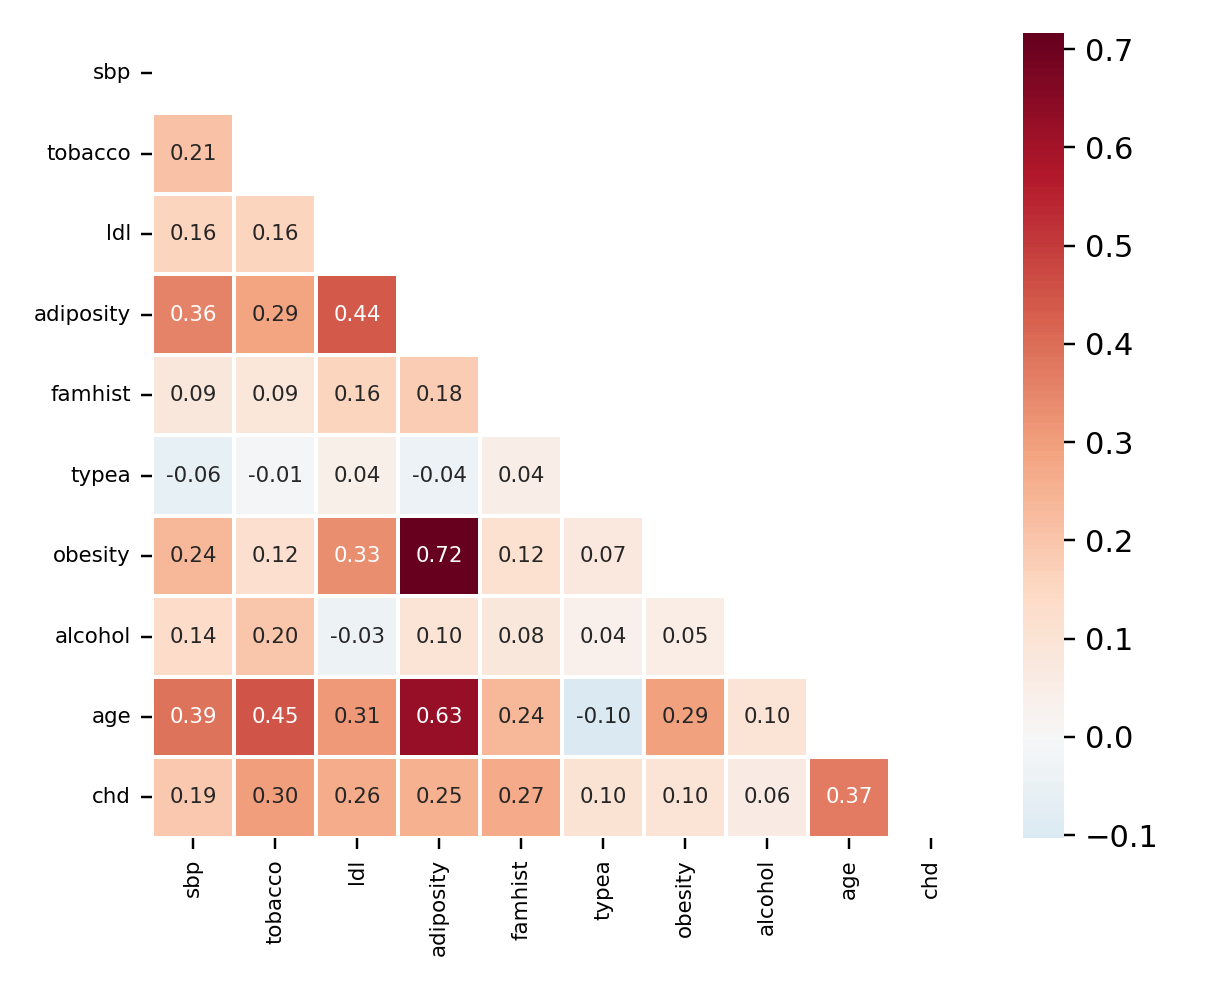
\includegraphics[width=\linewidth]{../exploratory_data_analysis/eda_output/fig_correlation_heatmap.png}
\caption{\footnotesize Pearson correlation matrix.}
\label{fig:corr}
\vspace{-8pt}
\end{wrapfigure}

\texttt{alcohol} ($r=0.06$) and \texttt{obesity} ($r=0.10$) are
the weakest predictors. A moderate positive correlation between
\texttt{adiposity} and \texttt{obesity} ($r=0.72$) suggests partial
multicollinearity, motivating ridge regularisation in Section~\ref{sec:lrrp}
\cite{hassan2022effectively, ogunpola2024machine}.
Violin plots stratified by CHD class confirm that \texttt{age}, \texttt{tobacco},
and \texttt{ldl} show the clearest class-conditional separation, while
\texttt{obesity} and \texttt{typea} distributions overlap substantially.

Log\,\textsubscript{1p}-transformation of the four dynamically identified
skewed features reduces their skewness markedly (Figure~\ref{fig:logtr}):
\texttt{alcohol} from 2.31 to 0.44, \texttt{tobacco} from 2.08 to 0.53,
\texttt{ldl} from 1.31 to 0.50, and \texttt{sbp} from 1.18 to 0.48.
These transformations are applied as a preprocessing option in the
modelling stages (Sections~\ref{sec:lrrp}--\ref{sec:oc}).

% ── Distribution analysis + log-transform ────────────────────────────────────
\begin{figure}[H]
\centering
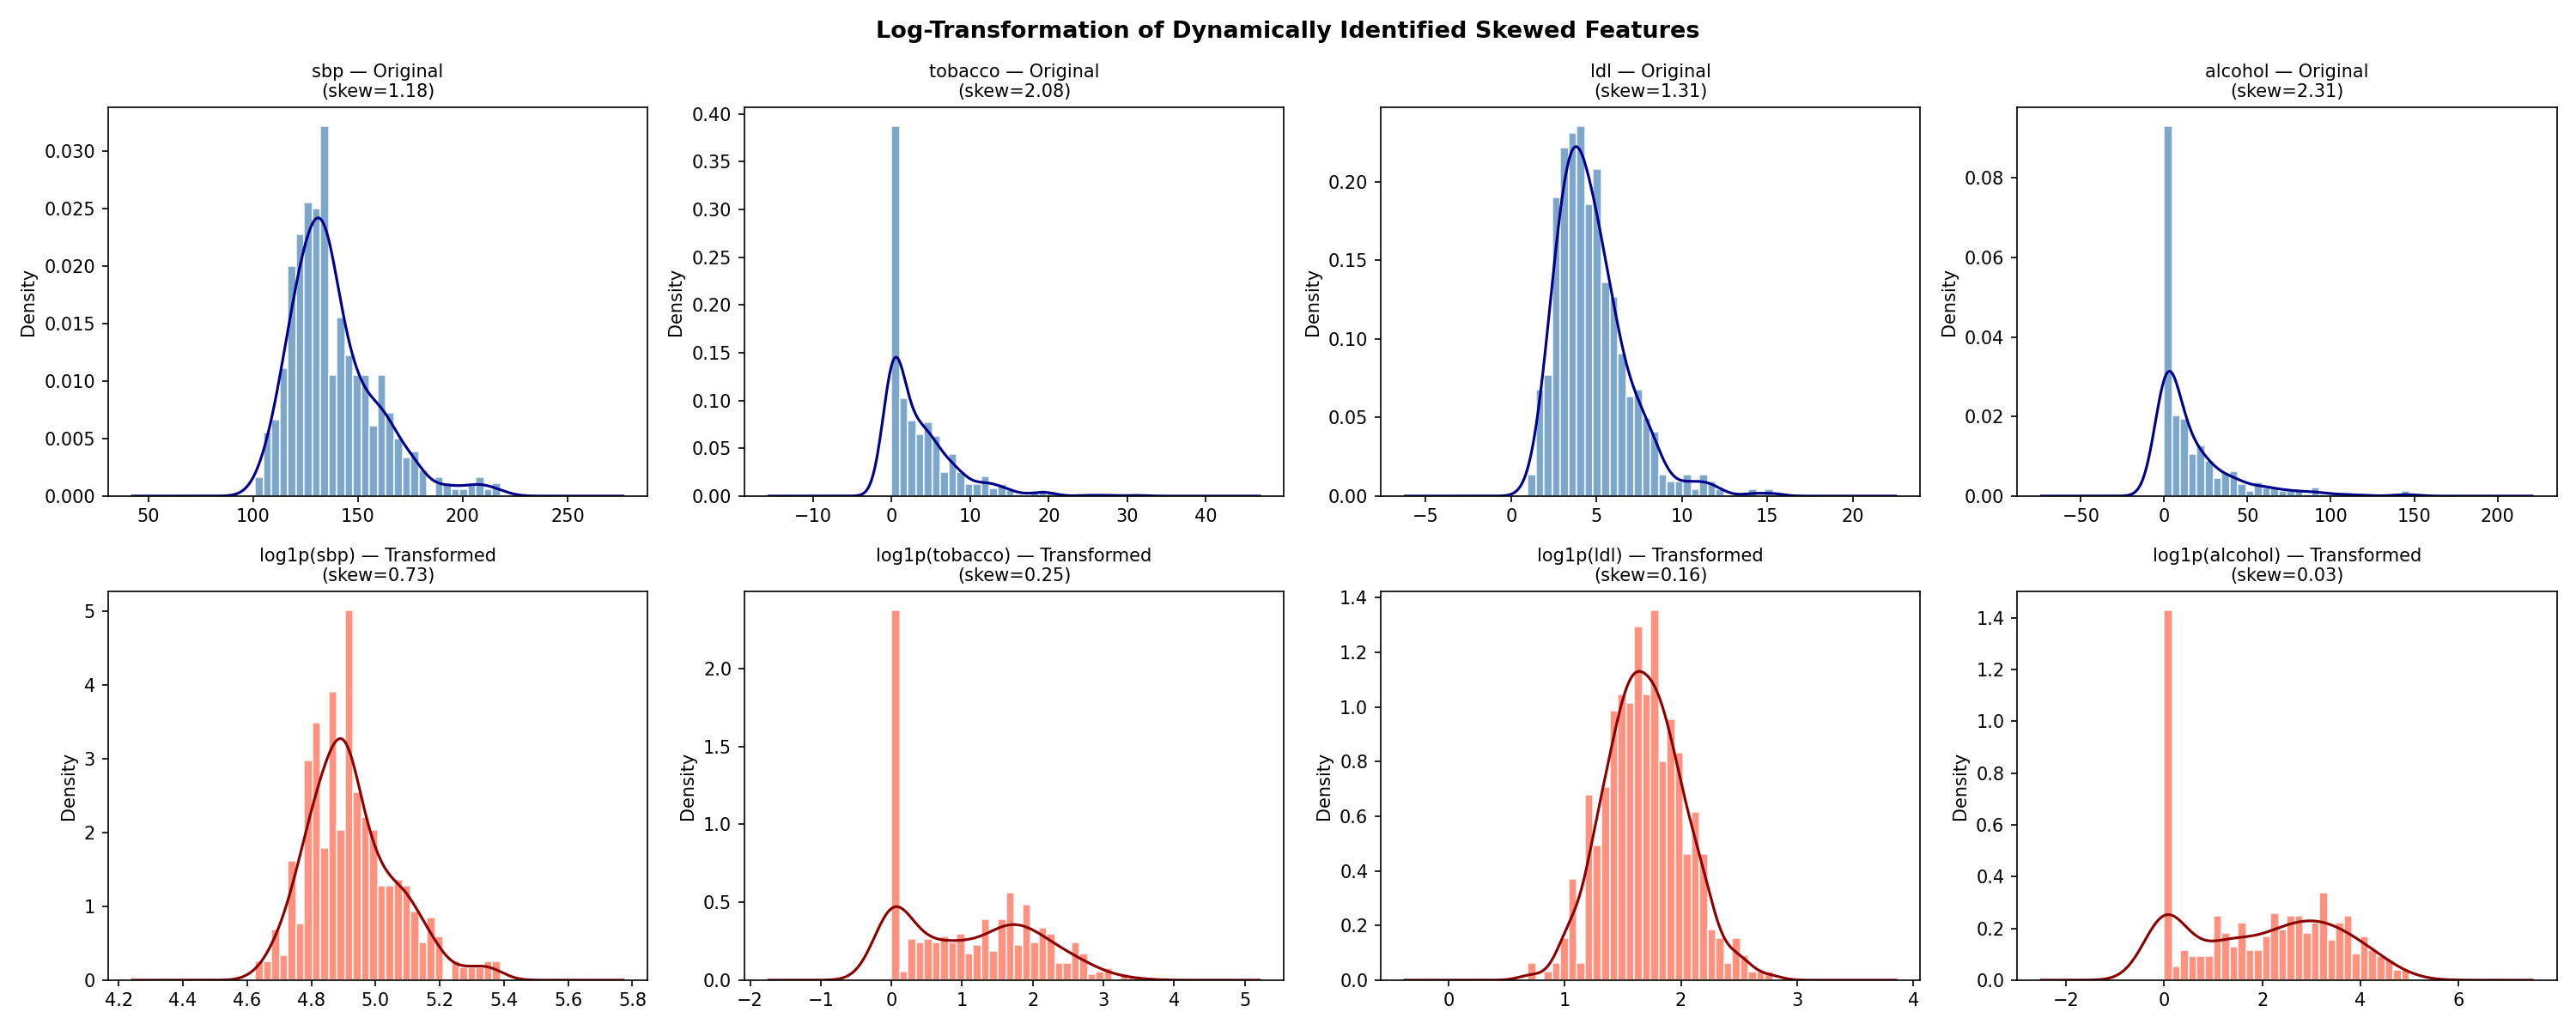
\includegraphics[width=\textwidth]{../exploratory_data_analysis/eda_output/fig_log_transformed_features.png}
\caption{\footnotesize Log\textsubscript{1p}-transformation of the
four dynamically identified skewed features.}
\label{fig:logtr}
\end{figure}

% ── Feature importance: text left, table right (in-flow minipages) ────────────
\noindent
\begin{minipage}[t]{0.50\linewidth}
\raggedright
Feature importance was assessed jointly using mutual information (MI) and
the ANOVA F-test \cite{elsofany2024proposed, ullah2024machine}. Using two
complementary criteria guards against misleading rankings from linear
assumptions alone. Table~\ref{tab:fi} shows the normalised scores: \texttt{age}
ranks first under both criteria, while \texttt{obesity} and \texttt{typea}
score lowest. These rankings directly inform the variable selection strategy
for the ridge logistic regression in Section~\ref{sec:lrrp}.
\end{minipage}\hfill
\begin{minipage}[t]{0.46\linewidth}
\centering
\captionof{table}{\footnotesize Normalised feature importance scores (ranked by mean).}
\label{tab:fi}
\vspace{2pt}
{\footnotesize
\begin{tabular}{@{}lrrr@{}}
\toprule
Feature    & MI   & ANOVA & Mean \\
\midrule
age        & 1.00 & 1.00  & 1.00 \\
tobacco    & 0.39 & 0.60  & 0.50 \\
famhist    & 0.43 & 0.48  & 0.46 \\
sbp        & 0.34 & 0.22  & 0.28 \\
ldl        & 0.00 & 0.45  & 0.22 \\
adiposity  & 0.00 & 0.41  & 0.21 \\
alcohol    & 0.16 & 0.00  & 0.08 \\
typea      & 0.07 & 0.04  & 0.06 \\
obesity    & 0.00 & 0.04  & 0.02 \\
\bottomrule
\end{tabular}}
\end{minipage}

% ── PCA ──────────────────────────────────────────────────────────────────────
\begin{figure}[h!]
\centering
\begin{minipage}{0.54\linewidth}
\centering
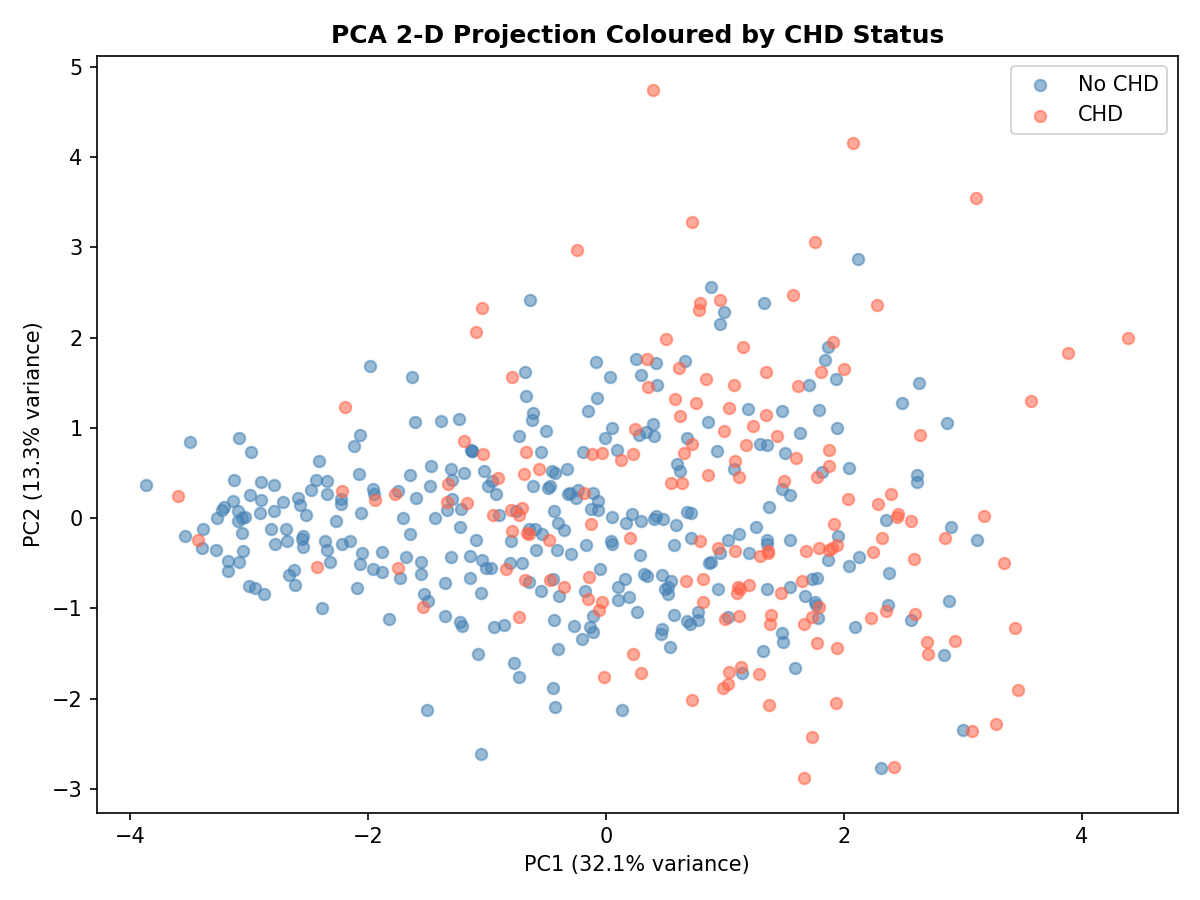
\includegraphics[width=\linewidth]{../exploratory_data_analysis/eda_output/fig_pca_scatter.png}
\caption{\footnotesize PCA 2-D projection coloured by CHD class.}
\label{fig:pca}
\end{minipage}\hfill
\begin{minipage}{0.42\linewidth}
\centering
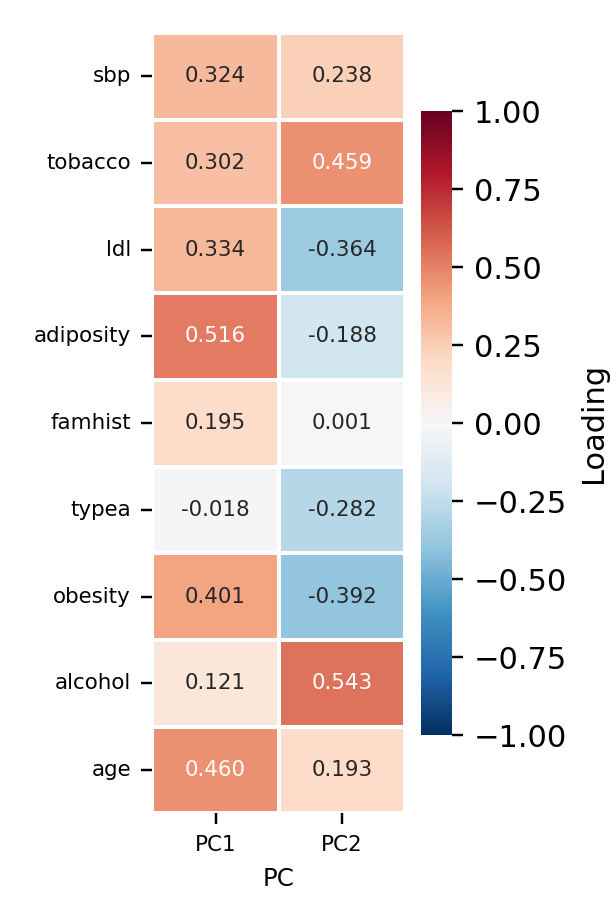
\includegraphics[width=\linewidth]{../exploratory_data_analysis/eda_output/fig_pca_loadings_heatmap.png}
\caption{\footnotesize PCA feature loadings (PC1 \& PC2).}
\label{fig:pcaload}
\end{minipage}
\end{figure}

PCA was applied to the standardised feature matrix
\cite{banerjee2025systematic}. PC1 explains 32.1\% of variance and loads
positively on \texttt{adiposity} (0.52), \texttt{age} (0.46), and
\texttt{obesity} (0.40) --- a latent \emph{metabolic risk} axis. PC2 is
driven by \texttt{alcohol} (0.54) and \texttt{tobacco} (0.46), reflecting a
\emph{lifestyle} axis. Seven components are needed to reach 90\% cumulative
variance, indicating moderate intrinsic dimensionality. The 2-D
projection (Figure~\ref{fig:pca}) shows partial but incomplete class
separation; the loadings heatmap (Figure~\ref{fig:pcaload}) confirms PC1
captures metabolic risk while PC2 captures lifestyle behaviours, motivating
non-linear classifiers in Section~\ref{sec:oc}.

% =============================================================================
\section{Logistic Regression with Ridge Penalty}
\label{sec:lrrp}
% =============================================================================

\noindent
\begin{minipage}[t]{0.50\linewidth}
\raggedright
Logistic regression with an L2 (ridge) penalty was chosen as the primary
interpretable classifier. The multicollinearity between \texttt{adiposity}
and \texttt{obesity} ($r=0.72$, Section~\ref{sec:eda}) motivates
regularisation: ridge shrinks correlated coefficients jointly without zeroing
any out \cite{borges2025logistic, hassan2022effectively}.

All nine features were retained. Preprocessing mirrors the EDA pipeline:
\texttt{famhist} encoded as 0/1; \texttt{sbp}, \texttt{tobacco},
\texttt{ldl}, and \texttt{alcohol} log\,\textsubscript{1p}-transformed;
all features standardised with \texttt{StandardScaler} (zero mean, unit
variance) so coefficient magnitudes are directly comparable.

The regularisation strength $C$ (inverse of $\lambda$) was selected by
stratified 5-fold cross-validation over the grid
$\{0.001, 0.01, 0.1, 1, 10, 100\}$ maximising AUC-ROC on an 80\,\%
training set. Table~\ref{tab:coef} lists the standardised coefficients of
the best model ($C=0.01$, CV-AUC$=0.760$).
\end{minipage}\hfill
\begin{minipage}[t]{0.46\linewidth}
\centering
\captionof{table}{\footnotesize Standardised coefficients of the ridge
logistic regression ($C=0.01$), sorted by $|\beta|$.}
\label{tab:coef}
\vspace{2pt}
{\footnotesize
\begin{tabular}{@{}lrr@{}}
\toprule
Feature    & $\hat{\beta}$ & $|\hat{\beta}|$ \\
\midrule
age        &  0.246 & 0.246 \\
famhist    &  0.205 & 0.205 \\
tobacco    &  0.198 & 0.198 \\
ldl        &  0.180 & 0.180 \\
typea      &  0.118 & 0.118 \\
adiposity  &  0.085 & 0.085 \\
sbp        &  0.080 & 0.080 \\
obesity    &  0.014 & 0.014 \\
alcohol    & $-$0.013 & 0.013 \\
\bottomrule
\end{tabular}}
\end{minipage}

\vspace{4pt}
The optimal $C=0.01$ implies strong regularisation, consistent with
multicollinear features reducing effective degrees of freedom.
\texttt{age} has the largest effect ($\hat{\beta}=0.246$), followed by
\texttt{famhist} ($0.205$) and \texttt{tobacco} ($0.198$), reinforcing
the EDA rankings. \texttt{obesity} and \texttt{alcohol} are almost fully
shrunk to zero, suggesting they contribute little beyond what \texttt{adiposity}
and \texttt{tobacco} already capture.

% ── ROC + confusion matrix ─────────────────────────────────────────────────
\begin{figure}[H]
\centering
\begin{minipage}{0.48\linewidth}
\centering
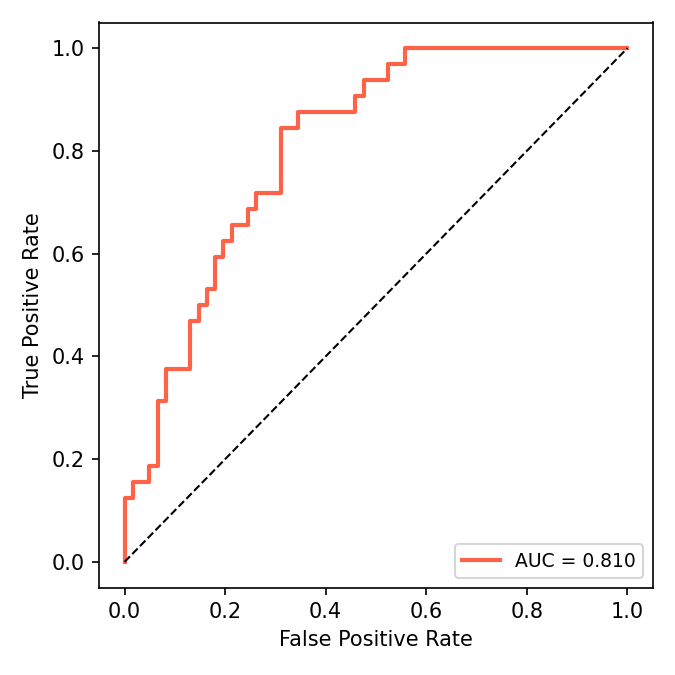
\includegraphics[width=\linewidth]{../logistic_regression_ridge_penalty/lrrp_output/fig_lrrp_roc_curve.png}
\caption{\footnotesize ROC curve for the ridge logistic regression
($C=0.01$) on the 20\,\% held-out test set.}
\label{fig:roc}
\end{minipage}\hfill
\begin{minipage}{0.48\linewidth}
\centering
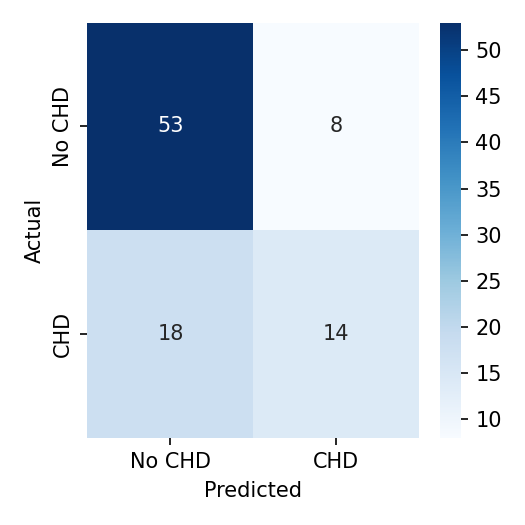
\includegraphics[width=\linewidth]{../logistic_regression_ridge_penalty/lrrp_output/fig_lrrp_confusion_matrix.png}
\caption{\footnotesize Confusion matrix at the 0.5 decision threshold
(test set, $n=93$).}
\label{fig:cm}
\end{minipage}
\end{figure}

On the held-out test set ($n=93$, 20\,\%) the model achieves
AUC\,=\,0.810, F1\,=\,0.52, and accuracy\,=\,0.72
(Table~\ref{tab:perf}). The confusion matrix (Figure~\ref{fig:cm}) reveals
that CHD recall is 0.44 versus No-CHD recall of 0.87, a consequence of the
1.89:1 class imbalance; the model tends to predict the majority class. AUC
of 0.810 is nevertheless substantially above the 0.5 random baseline and
competitive with published benchmarks on similar datasets
\cite{rehman2025predicting, ogunpola2024machine}.

\begin{table}[h!]
\centering
\caption{\footnotesize Test-set performance of the ridge logistic regression.}
\label{tab:perf}
\vspace{2pt}
{\footnotesize
\begin{tabular}{@{}lcccc@{}}
\toprule
Model & AUC-ROC & F1 & Precision & Recall \\
\midrule
Ridge LR ($C=0.01$) & 0.810 & 0.52 & 0.64 & 0.44 \\
\bottomrule
\end{tabular}}
\end{table}

% =============================================================================
\section{Alternative Classifiers}
\label{sec:oc}
% =============================================================================

% TODO: Complete after implementing other_classifiers/oc.py
%
% Structure:
%   - Classifier selection motivation (tree-based, kernel-based, ensemble)
%   - Cross-validated comparison table (Accuracy, AUC, F1, Recall) — minipage
%   - Best classifier: tuning procedure, final results, discussion

\noindent\textit{This section will be completed upon implementation of
\texttt{other\_classifiers/oc.py}.}

% =============================================================================
% References
% =============================================================================
\newpage
\bibliographystyle{plainnat}
\bibliography{references}

% =============================================================================
% Appendix
% =============================================================================
\newpage
\begin{appendices}

\section{Code Replication Instructions}

The full source code is available on GitHub:

\begin{center}
\url{https://github.com/manpreet-sangha/predict_coronary_heart_disease}
\end{center}

\noindent The interactive live dashboard is accessible at:

\begin{center}
\url{https://predict-coronary-heart-disease.streamlit.app/}
\end{center}

\subsection*{Local Setup}

\begin{enumerate}
    \item Clone the repository and enter the project directory.
    \item Create and activate a virtual environment:
          \texttt{python -m venv .venv} then \texttt{.venv\textbackslash Scripts\textbackslash activate} (Windows).
    \item Install dependencies: \texttt{pip install -r requirements.txt}
    \item Run the full pipeline: \texttt{python chd\_main.py}\\
          Outputs saved to \texttt{exploratory\_data\_analysis/eda\_output/}.
    \item Launch dashboard: \texttt{streamlit run app.py}
\end{enumerate}

\noindent Python~$\geq$\,3.10 required. Key packages: \texttt{pandas\,$\geq$\,2.0},
\texttt{scikit-learn\,$\geq$\,1.4}, \texttt{streamlit\,$\geq$\,1.35},
\texttt{plotly\,$\geq$\,5.20}.

\end{appendices}

\end{document}
